\documentclass[twocolumn,showpacs]{revtex4-1}
%\usepackage{dblfloatfix}
\usepackage{subcaption} \usepackage{graphicx} \usepackage{amsmath}
\graphicspath{{./fig/}}
%\def\input@path{{./src/}}

\bibliographystyle{revtex}
\begin{document}

\title[Beyond Nuclear Pasta]{Beyond Nuclear Pasta: Phase Transitions
  and Neutrino Opacity of New Pasta Phases}

\author{P. N. Alcain, P. A. Gim\'enez Molinelli and C. O. Dorso}

\affiliation{Departamento de F\'isica, FCEyN, UBA and IFIBA, Conicet,
Pabell\'on 1, Ciudad Universitaria, 1428 Buenos Aires, Argentina}
\affiliation{IFIBA-CONICET}

\date{\today} \pacs{PACS 24.10.Lx, 02.70.Ns, 26.60.Gj, 21.30.Fe}

\begin{abstract}
En este capítulo tratamos las distintas escalas de longitud dentro de
la dinamica de los nucleones en condiciones acordes a las de la corteza de las estrellas de neutrones, estudiando materia simétrica en isospín (igual cantidad de protones y neutrones) a densidades menores a la de saturación para 5000 partículas.
Variando la temperatura encontramos una tranisición de fase sólido-líquido que se puede caracterizar también como una transición morfológica.
Para temperaturas más altas que la de la transición de fase estudiamos la opacidad de los neutrinos y encontramos que en la fase líquida el \emph{scattering} de los neutrinos de bajo momento se mantiene elevado, incluso con morfologías que son significativamente diferentes a las de la pasta nuclear tradicional.\end{abstract}

\maketitle

\subsection{Transición de fase}
\subsubsection{Transición de fase termodinámica}

La figura~\ref{fig:energy} presenta la energía como función de la temperatura (curva calórica) para distintas densidades.
Cada una de estas densidades exhibe una discontinuidad en la energía para ciertas temperaturas, una señal de una transición de fase de primer orden.
Esta transición puede ser confirmada y caracterizada como de sólido-líquido observando el coeficiente de Lindemann. Por ejemplo, mostramos el coeficiente de Lindemann junto a la energía para $\rho=0.05\,\text{fm}^{-3}$ en la figura~\ref{fig:lind-energ}.
Esta figura muestra que las discontinuidades en las energía y en el coeficiente de Lindemann están a la misma temperatura.
Éstas dos son características de la transición de fase sólido-líquido.

\begin{figure}[h!]  \centering
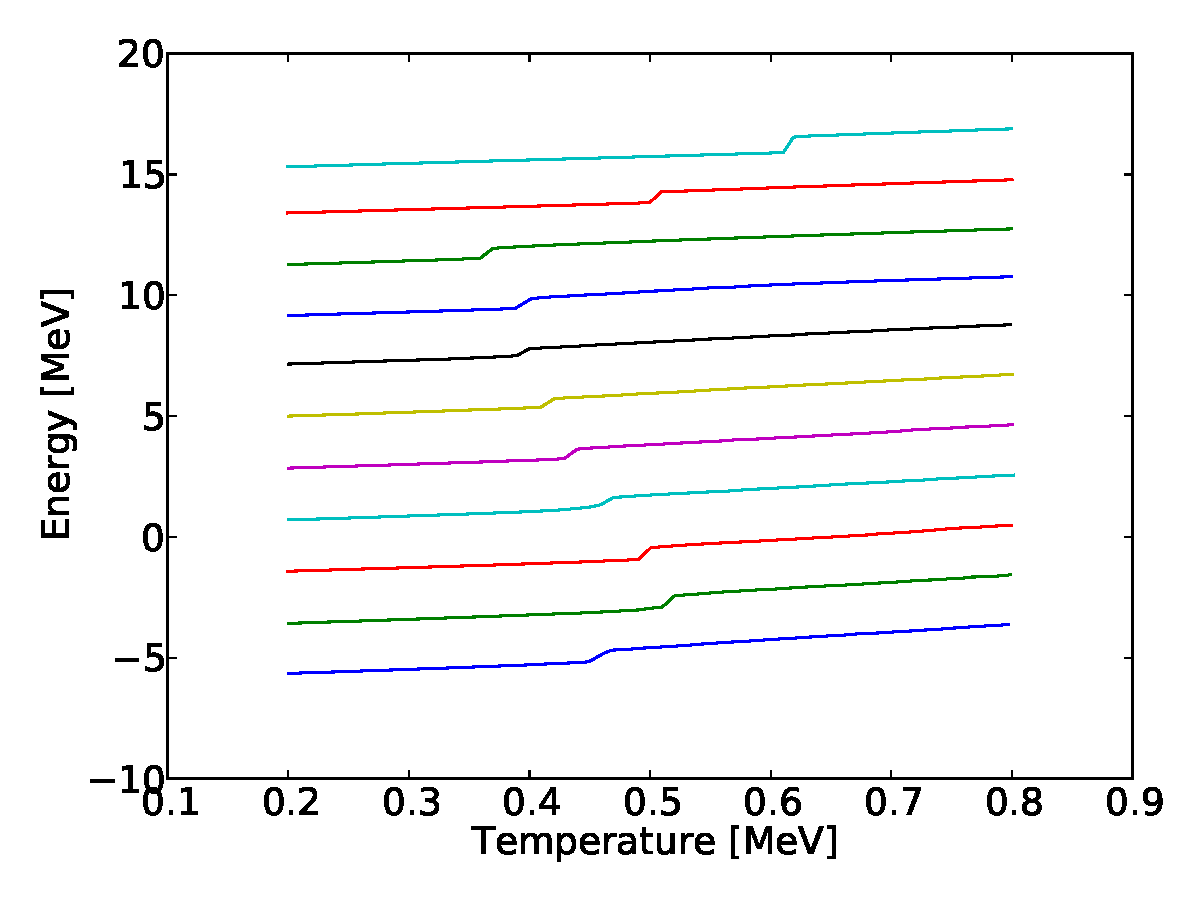
\includegraphics[width=\columnwidth]{energy.pdf}
\caption{Energía como función de la temperatura para distintas densidades.
  Observamos una discontinuidad en el rango desde $T_l=0.35\,\text{MeV}$ a $T_h=0.65\,\text{MeV}$, dependiendo de la densidad.
  Esto es una señal de una transición de fase.
  En la figura, las densidades van de $\rho=0.03\,\text{fm}^{-3}$ a $\rho=0.13\,\text{fm}^{-3}$, incrementando $\Delta\rho=0.01\,\text{fm}^{-3}$ hacia arriba.}
\label{fig:energy}
\end{figure}

\begin{figure}[h!]  \centering
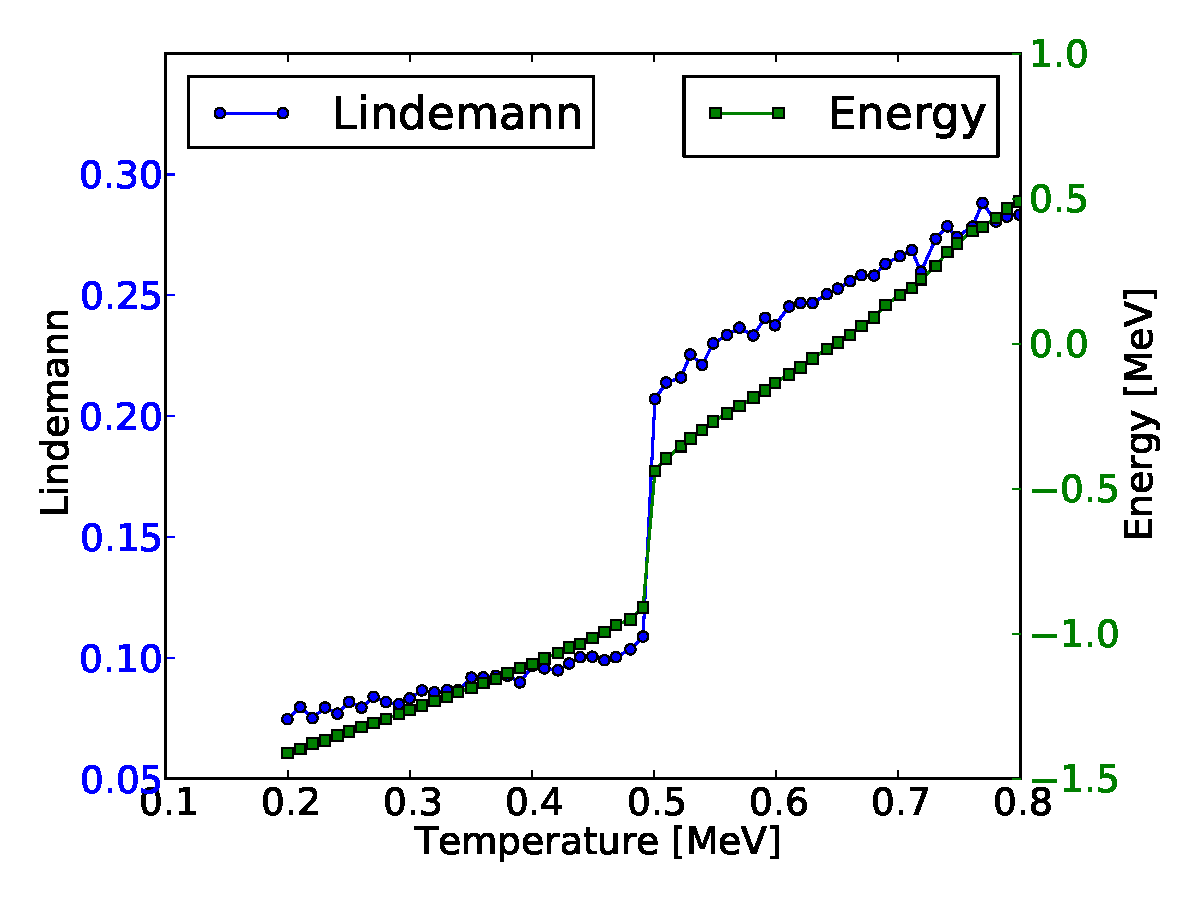
\includegraphics[width=\columnwidth]{lind-energ.pdf}
\caption{Coeficiente de Lindemann y energía como función de la temperatura para una densidad, $\rho=0.05\,\text{fm}^{-3}$.
  El cambio abrupto en su valor es una señal de una transición de fase sólido-líquido.
  Podemos ver que ambas discontinuidades están a la misma temperatura.}
\label{fig:lind-energ}
\end{figure}

En la figura~\ref{fig:rdf} mostramos la función de distribución de pares para tres densidades distintas: $\rho=0.03\,\text{fm}^{-3}$ (\emph{spaghetti}), $\rho=0.05\,\text{fm}^{-3}$ (\emph{lasagna}) y $\rho=0.08\,\text{fm}^{-3}$ (túneles), inmediatamente sobre y bajo la temperatura de transición, así como una foto del sistema en la fase de temperatura alta.
Como los primeros picos (correspondientes a los primeros vecinos) están en la misma posición más allá de la temperatura, comcluimos que el orden corto está present tanto sobre como bajo la transición.
Sin embargo los los picos de los terceros vecinos, distintivos de las fases sólidas, desaparecen a medida que la temperatura aumenta más allá de la transición.
El orden de muy largo ranto también sobrevivie a la transición, como discutimos más adelante en la sección~\ref{very_long}

\begin{figure*}[floatfix]
  \centering
  \begin{subfigure}[h!]{0.95\columnwidth}
    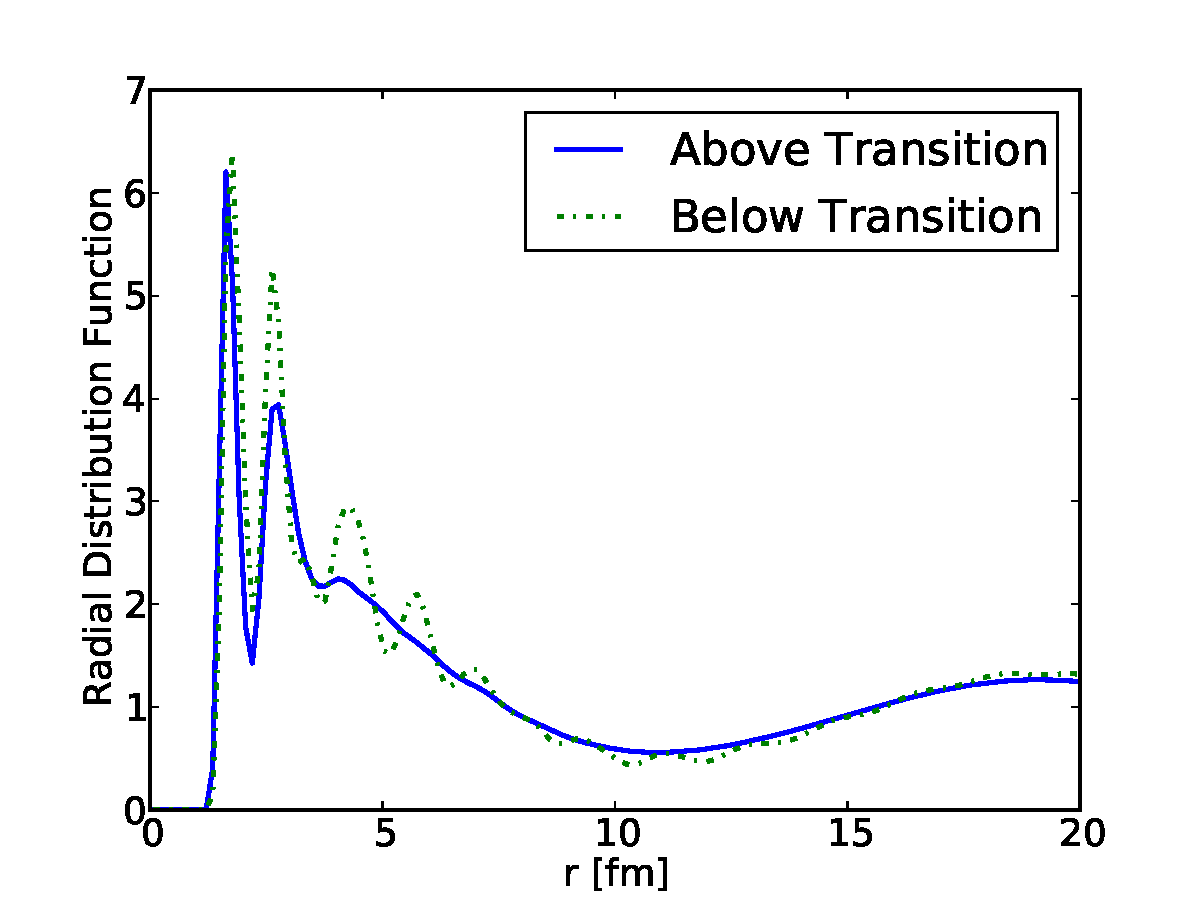
\includegraphics[width=\columnwidth]{rdf_0-03.pdf}
    \caption{Función de distribución de pares para $\rho=0.03\,\text{fm}^{-3}$}
  \end{subfigure}
  \begin{subfigure}[h!]{0.70\columnwidth}
    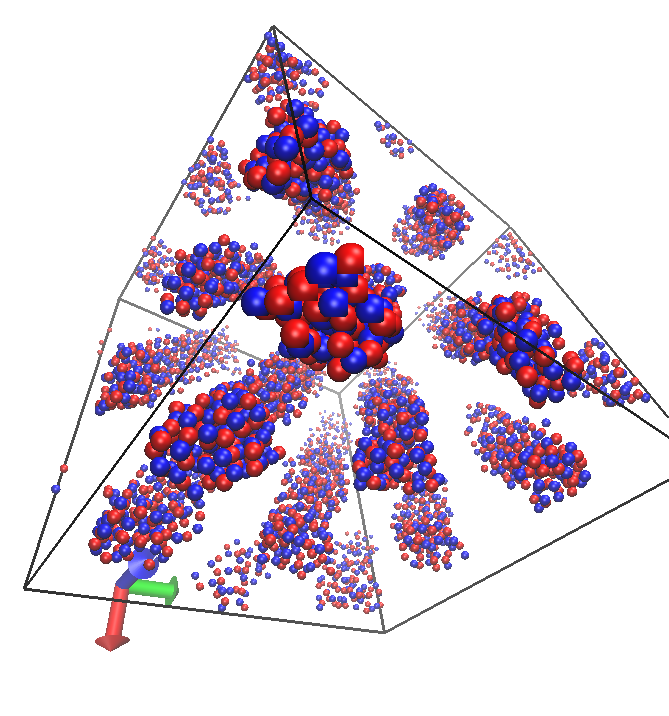
\includegraphics[width=\columnwidth]{morph_0-03_0-47.png}
    \caption{Foto del sistema en la fase líquida para $\rho=0.03\,\text{fm}^{-3}$}
  \end{subfigure}
  \begin{subfigure}[h!]{0.95\columnwidth}
    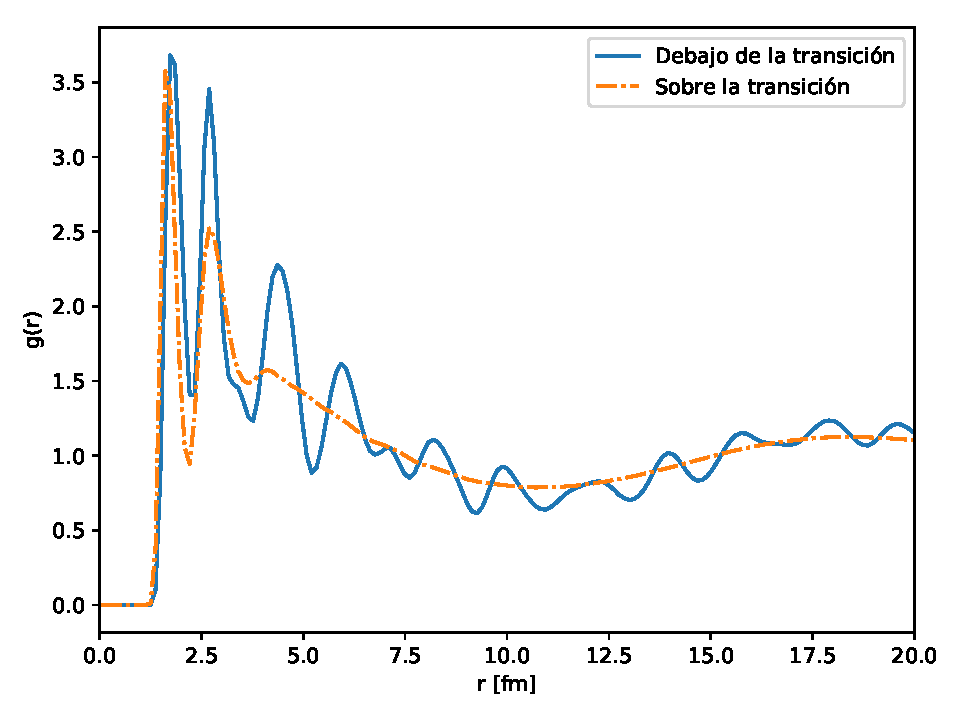
\includegraphics[width=\columnwidth]{rdf_0-05.pdf}
    \caption{Función de distribución de pares para $\rho=0.05\,\text{fm}^{-3}$}
  \end{subfigure}
  \begin{subfigure}[h!]{0.70\columnwidth}
    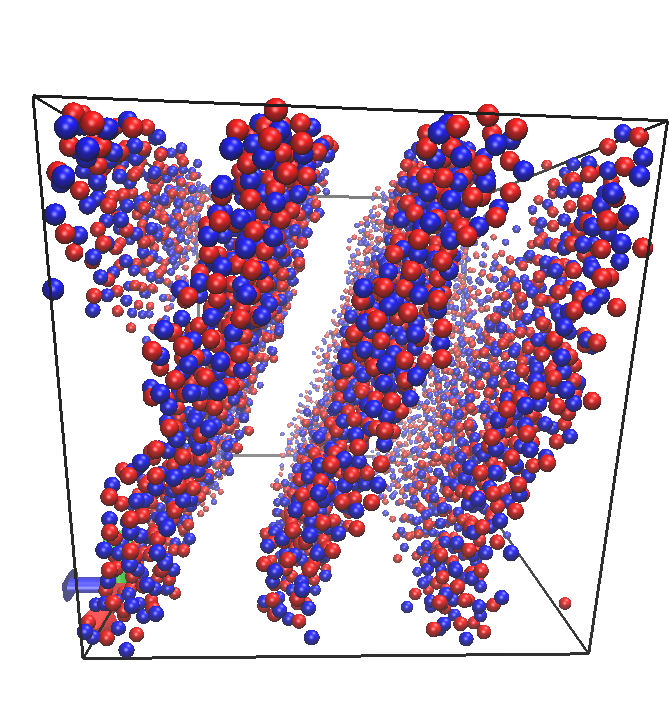
\includegraphics[width=\columnwidth]{morph_0-05_0-50.png}
    \caption{Foto del sistema en la fase líquida para $\rho=0.05\,\text{fm}^{-3}$}
  \end{subfigure}
  \begin{subfigure}[h!]{0.95\columnwidth}
    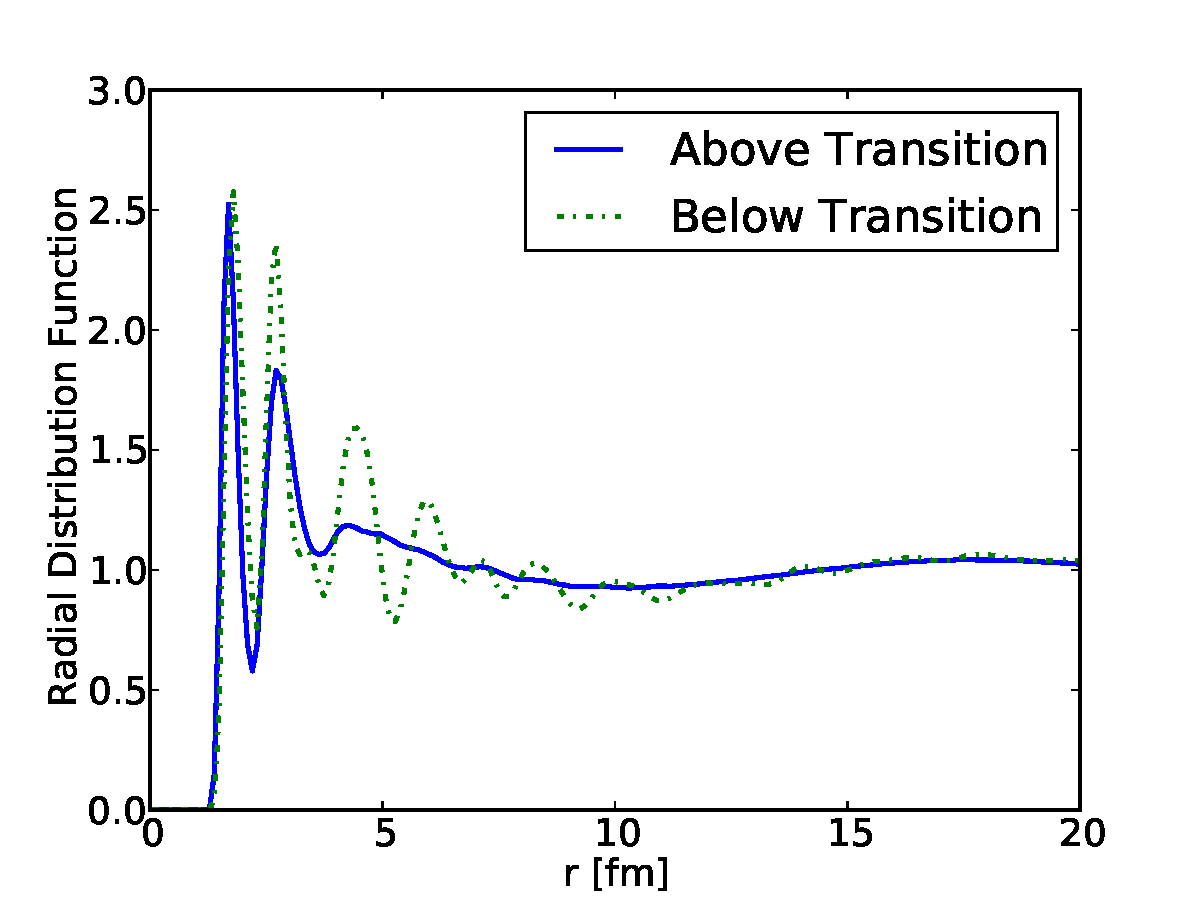
\includegraphics[width=\columnwidth]{rdf_0-08.pdf}
    \caption{Función de distribución de pares para $\rho=0.08\,\text{fm}^{-3}$}
  \end{subfigure}
  \begin{subfigure}[h!]{0.70\columnwidth}
    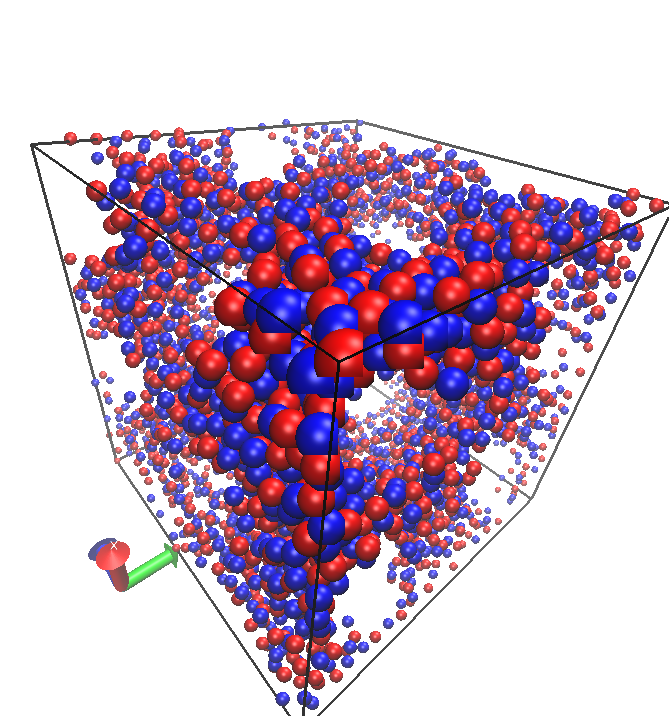
\includegraphics[width=\columnwidth]{morph_0-08_0-42.png}
    \caption{Foto del sistema en la fase líquida para $\rho=0.08\,\text{fm}^{-3}$}
  \end{subfigure}
  \caption{Función de distribución de pares para distintas densidades, tanto debajo como sobre la temperatura de transición, y foros del sistema en la fase líquida.
Aunque los pirmeros picos de la distribución están en las mismas posiciones para ambas temperaturas, los picos siguientes, que exhiben un orden de rango largo típico de los sólidos, sólo están presentes por debajo de la temperatura de transición.}
  \label{fig:rdf}
\end{figure*}

\subsubsection{Transición de fase morfológica}
Cuando observamos los funcionales de Minkowski, particularmente la característica de Euler y el ancho medio, observamos que también hay una temperatura ``crítica'' en la cual ambas magnitudes exhiben una transición abrupta.
Mostramos, como un ejemplo, estas magnitudes como función de la temperatura para la densidad
$\rho=0.05\,\text{fm}^{-3}$ en la figura~\ref{fig:euler-curv}.
Como esta transición está señalada por los observables morfológicos, concluimos que es una transición también morfológica.
\todo[inline]{Explicar que es por los agujeros}

\begin{figure}%[H]
  \centering 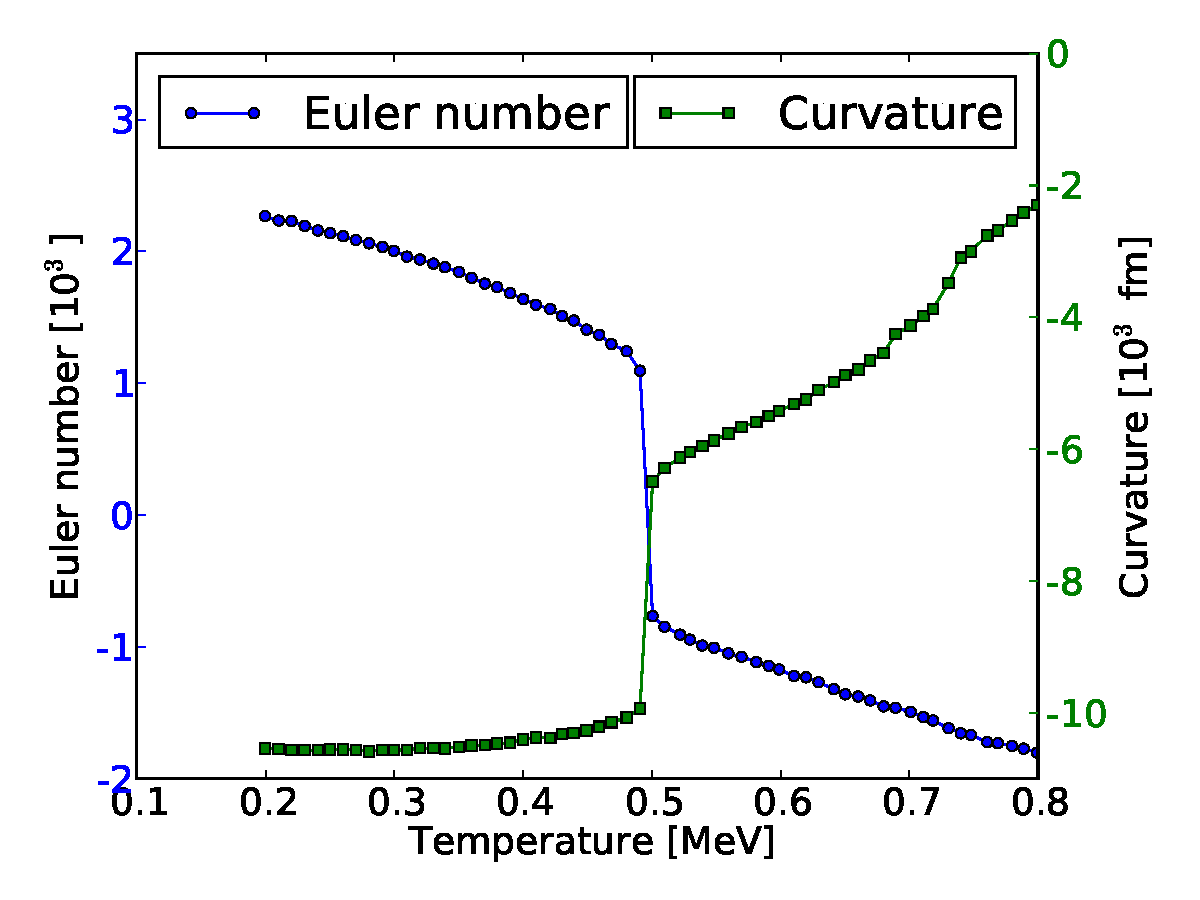
\includegraphics[width=\columnwidth]{euler-curv.pdf}
  \caption{Número de Euler y ancho medio para $\rho=0.05\,\text{fm}^{-3}$.
    Observamos una transición abrupta para ambas funcionales de Minkowski.}
  \label{fig:euler-curv}
\end{figure}

Estas señales de una transición sólido-líquido (discontinuidad en la energía y en el coeficiente de Lindemann) y morfológica (discontinuidad en las funcionales de Minkowski) se producen a la misma temperatura de transición, como se puede observar en el diagrama de fases de la figura~\ref{fig:critical_temperature}.
Esto significa que, a medida que el sistema es enfriado a un volumen fijo, sufre una transición termodinámica y morofológica a la misma temperatura.

\begin{figure}[floatfix]  \centering
  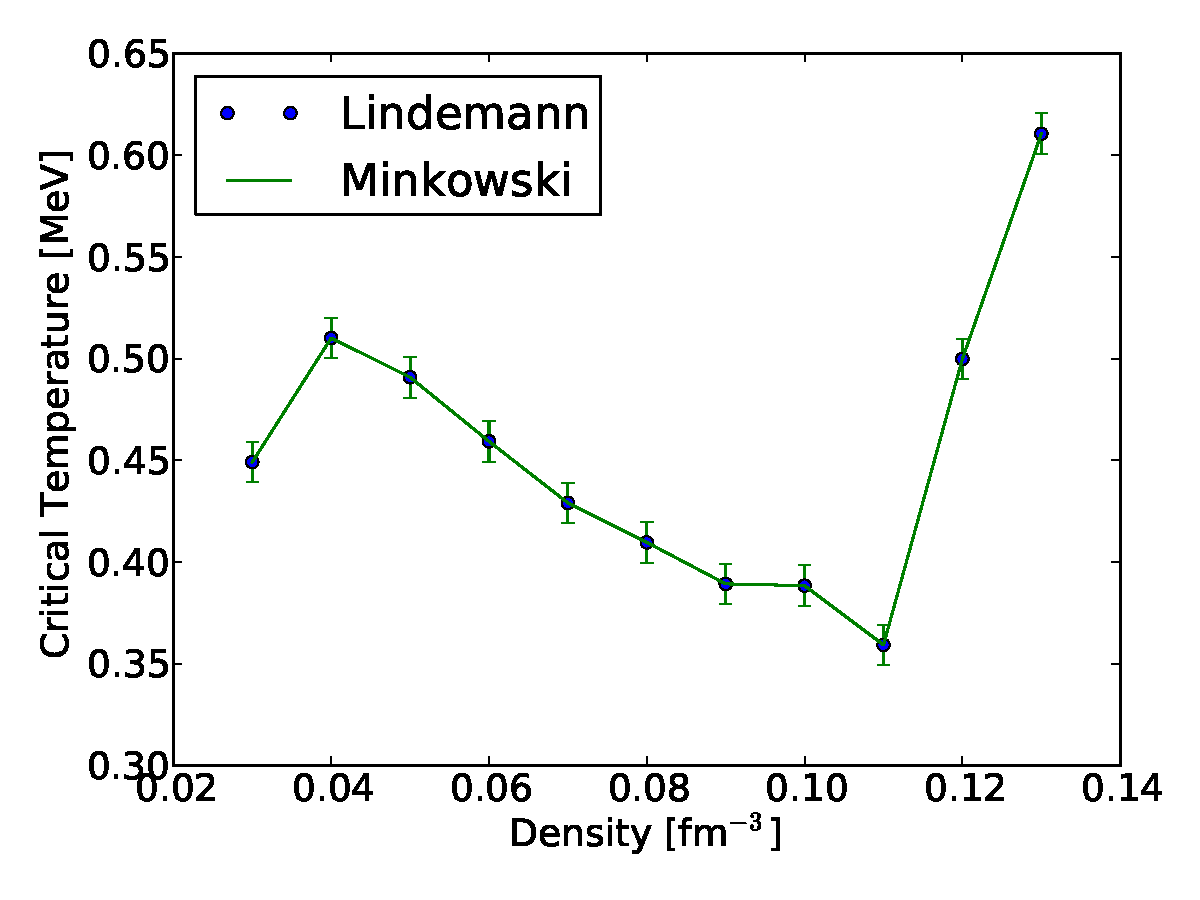
\includegraphics[width=\columnwidth]{critical_temperature.pdf}
  \caption{Temperatura crítica como función de la densidad.
    Observamos la superposición entre la temperatura crítica de las funcionales de Minkowski y el coeficiente de Lindemann.}
  \label{fig:critical_temperature}
\end{figure}


\subsection{Comportamiento de muy largo rango}
  \label{very_long}
  \input{src/very_long}

\subsection{Neutrino transport properties}
  \label{transport}
  \input{src/transport}

\subsection{Properties of non-traditional pasta}
  \label{unusual_pasta}
  \input{src/unusual_pasta}

\section{Discussion and concluding remarks}
  \label{discussion}
  \input{src/discussion}

\begin{acknowledgments}
  C.O.D. is a member of the Carrera de Investigador CONICET, work
  partially supported by CONICET Grant PIP0871. P.G.M. and P.N.A.  by
  a CONICET grant. The three-dimensional figures were prepared using
  Visual Molecular Dynamics~\cite{VMD}.
\end{acknowledgments}

\begin{thebibliography}{99}
  \input{src/bibliography}
\end{thebibliography}
\end{document}
